\section{Question 1}

\subsection{The Question}

\begin{flushleft}

Create a blog-term matrix.  Start by grabbing 100 blogs; include:

\vspace{10pt}
\url{http://f-measure.blogspot.com/}

\url{http://ws-dl.blogspot.com/}

\vspace{10pt}
and grab 98 more as per the method shown in class.

Use the blog title as the identifier for each blog (and row of the
matrix).  Use the terms from every item/title (RSS) or entry/title
(Atom) for the columns of the matrix.  The values are the frequency
of occurrence.  Essentially you are replicating the format of the
``blogdata.txt'' file included with the PCI book code.  Limit the
number of terms to the most ``popular'' (i.e., frequent) 500 terms,
this is *after* the criteria on p. 32 (slide 7) has been satisfied.

Create a histogram of how many pages each blog has (e.g., 30
blogs with just one page, 27 with two pages, 29 with 3 pages and 
so on).

\end{flushleft}


\subsection{The Answer}



RSS and Atom feeds are an XML-based syndication format that are used to organized all blogs so that they can be easily be broken down into posts without the need for complicated parsing. The link to the pages containing the RSS or Atom feed can be typically found in the webpage of the blog itself. This is the link that contains all the blog posts and will be used to create the blog matrix data. 

The code provided in the book \cite{PCI} contains many useful python functions and a script that generates a feed vector based on a list of feed URLs. However, the links provided as input must be to the RSS/Atom feed itself, rather than the blog. In addition, paged blog feeds must be provided in seperate links for each page. Therefore there is some preconditioning that must be done to obtain the data necessary to provide to this script. 

The assignment specifies that of the 100 blog posts the following must be included:

\vspace{10pt}
\url{http://f-measure.blogspot.com/}

\url{http://ws-dl.blogspot.com/}

\vspace{10pt}

and 98 other blogs from blogspot. In practice more than 100, approximately 120, blogs were collected to prevent from falling under the required 100 if errors in etracting the feed occured. The most common error presented was that certain blog required the reader to be logged in with their Google account, which made programmically retrieving the feed more complicated. Such blogs occured consistently at 2% - 3%, so a larger number was sampled then the blog matrix prunned to the required size. 


However, the remaining blogs must be selected at random from blogspot. This is addressed by using the link 

\vspace{10pt}
\url{https://www.blogger.com/next-blog?navBar=true&blogID=8145271598519191285}

\vspace{10pt}

that is requested when the ``Next'' button is pressed at the top of any blog. This automatically generates a new blog as a response to the request. Therefore, by making repeated requests to this URL the response received will always be different and random, for the most part. 

The ``Next'' button allows us to collect the URLs of blogs, but the main objective is to collect RSS/Atom feed URL. The response html was parsed using BeautifulSoup and the link to the Atom feed extracted, the Atom feed seemed easier to find the paged link. Once the first link was extracted a request wa made to that URL and from the response the next page link was extracted. This process was repeated until all the pages of the feed were collected. The links were all appended to a file that would be feed to the code provided by the book \cite{PCI}. A comma seperated file was created that contain the title and number of pages each blog contained in it. This is used later to produce the histogram of feed pages. 


\lstset{
    language=Python,
    label=code:q1,
    caption={Python module to collect Atom feed links from blogs}
}
\lstinputlisting{../q1/getBlogs.py}

The above Python script contains all the functions that are used to fetch a random blog, grab the Atom feed link and retrieve the paged feed links. The collection of Atom feed links, which link to each page of the feed, is saved in a file ``feedlist.txt'' that is used by the ``generatefeevector.py'' script to produce the blog matrix. In addition to this another file, ``feedstats.txt'', is created that contains the title of each blog and the number of pages the Atom feed contains. 


The code provided in the PCI book \cite{PCI} takes ``feedlist.txt'' as input and generates a blog matrix where every column is a word from a blog which adheres to this restriction:


\begin{lstlisting}
frac=float(bc)/len(feedlist)
  if frac>0.1 and frac<0.5:
\end{lstlisting}


Despite naive this restriction is accepted but the number of terms is limited to the top 500. To achieve this a small modification was required. The words were collected with their respective frequency value and then sorted. From the resulting list the top 500 terms were used.


\begin{lstlisting}
wordrank = []
for (w, bc) in apcount.items():
    frac = float(bc) / len(feedlist)
    if frac > 0.1 and frac < 0.5:
        wordrank.append((w,frac))

wordlist = []
# sort list based on frequency
wordrank.sort(key=lambda tup:tup[1], reverse=True)
for i in range(500):
    wordlist.append(wordrank[i][0].encode('ascii'))

\end{lstlisting}

A histogram of the number of feed pages can be easily generate from the data in ``feedstats.txt''. The data was stored in a comma seperated value format with all string enclosed in quotation marks to facilitate the file reading required by R.

The histogram function in R takes a vector of values and generates a frequency histogram with a default number of bins, usually 10. This is convenient, but produces bars for a range of integer values, e.g. 30 blogs have between 1 and 10 pages, 26 blogs have between 11 and 20 pages. However the desired results is one unit intevals, e.g., 30 blogs with just one page, 27 with two pages, 29 with 3 pages and so on. To achieve this we must specify the number of bins that we want to be produced in the histogram. This depends on the number of distinct values that occur.   In the case that each blog has a different number of pages this value is equal to the number of blogs and therefore we can use that as an upper bound.

\lstset{
    language=R,
    label=code:q1,
    caption={R script to produce histogram and density plot}
}
\lstinputlisting{../q1/math.r}

The expected outcome from intuition is that the histogram will follow a power-law trend where there are many blogs that contain few pages, at least one, but there are very few that have many pages. This result seems reasonable from previous assignments, but it is interesting if this simple ``many-few, few-many'' approach true characterizes the data, or is a useful approximation. 

\begin{wrapfigure}{r}{0.5\textwidth}
  \vspace{-20pt}
  \begin{center}
    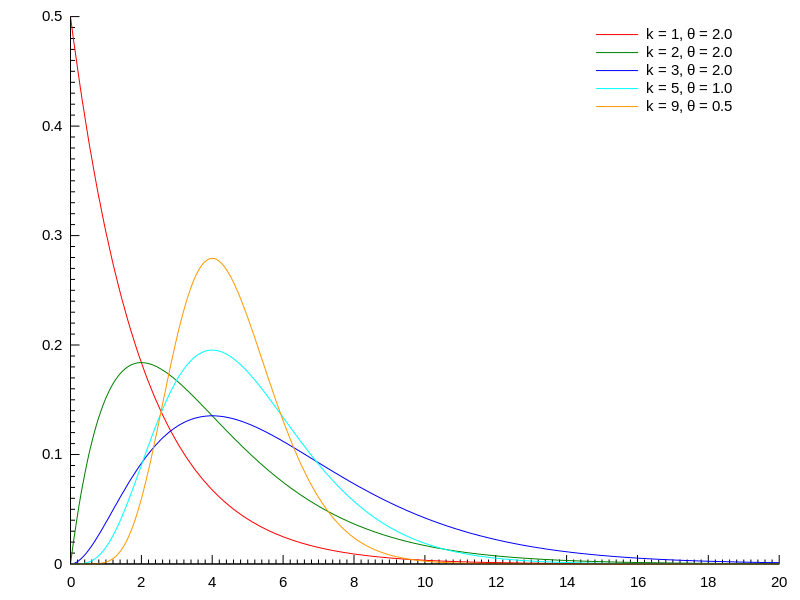
\includegraphics[width=0.5\textwidth]{gamma}
  \end{center}
  \vspace{-20pt}
  \caption{Gamma distributions}
  \vspace{-10pt}
\end{wrapfigure}



There is the possibility that there are very few bloggers that only have one page of feeds. Assuming someone was motivated to start blogging they would be very active in the beginning and write a substantial number of posts, enough for a few pages. Then the hype dies off and port become more infrequent and only the few committed bloggers stay active enough to collect many pages. But most people would write at least a few pages, meaning that the bulk of bloggers have some in between 1 or 2 pages and many pages. This is known as the Gamma distribution

The Gamma distribution describes a family of distributions, each with a different shape based on the parameter values. The known power-law distribution is a special case of the Gamma distribution. The Gamma distribution has the characteristic that it does not take negative values and is infinite in the positive direction. This is in contrast to the normal distribution that is defined for negative values. In this application a negative number of pages has no meaning and the Gamma distribution is the appropriate choice. Using the information from a useful blog post \cite{Rplots} we can create a histogram of the data and overlay the corresponding Gamma function fitted to the data's statistical modes, i.e. the mean and variance.
The following graphs show the histogram of the data as well as the fitted Gamma distribution.


\begin{figure}
\centering
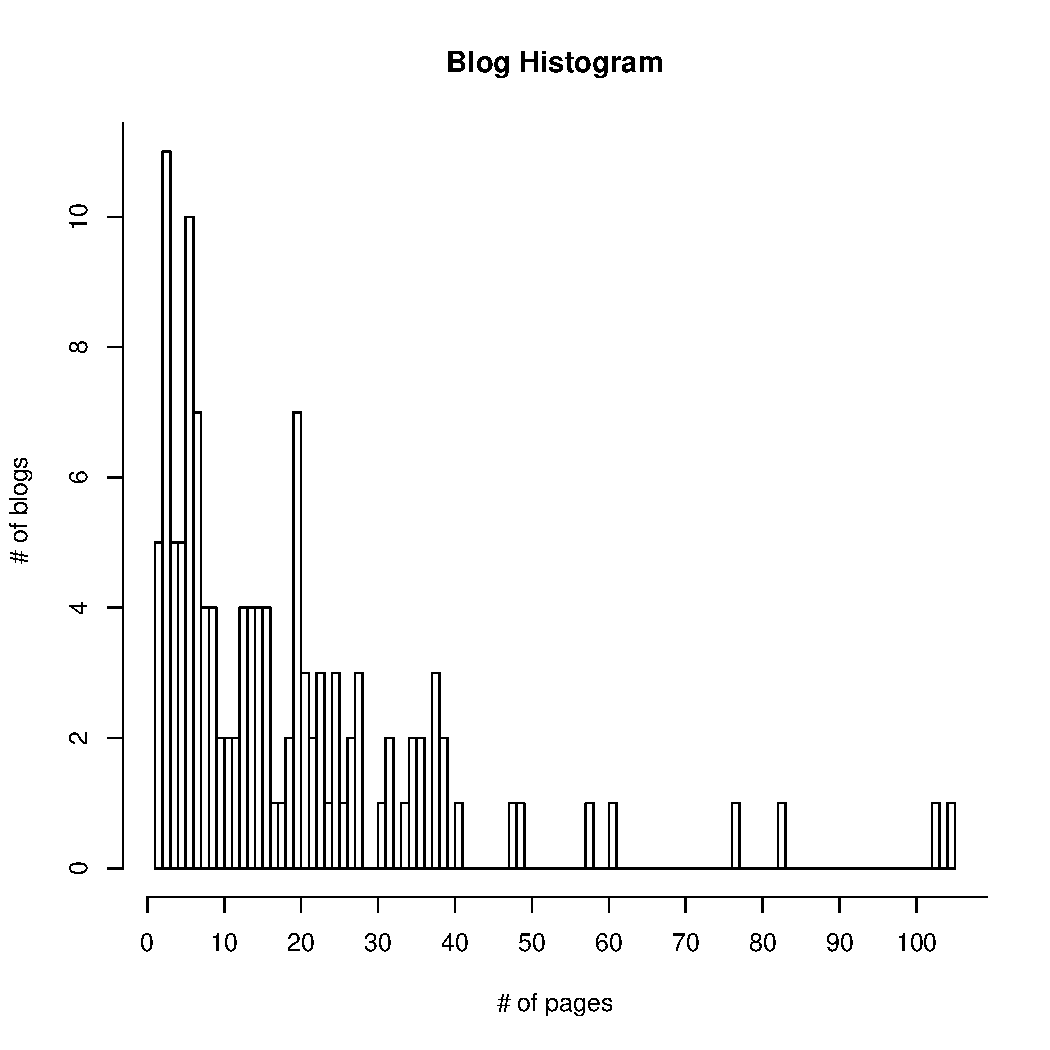
\includegraphics[width=.8\textwidth]{../q1/freqHist.pdf}
\caption{Frequency Histogram (bins = no. blogs)}
\end{figure}



\begin{figure}
  \centering
  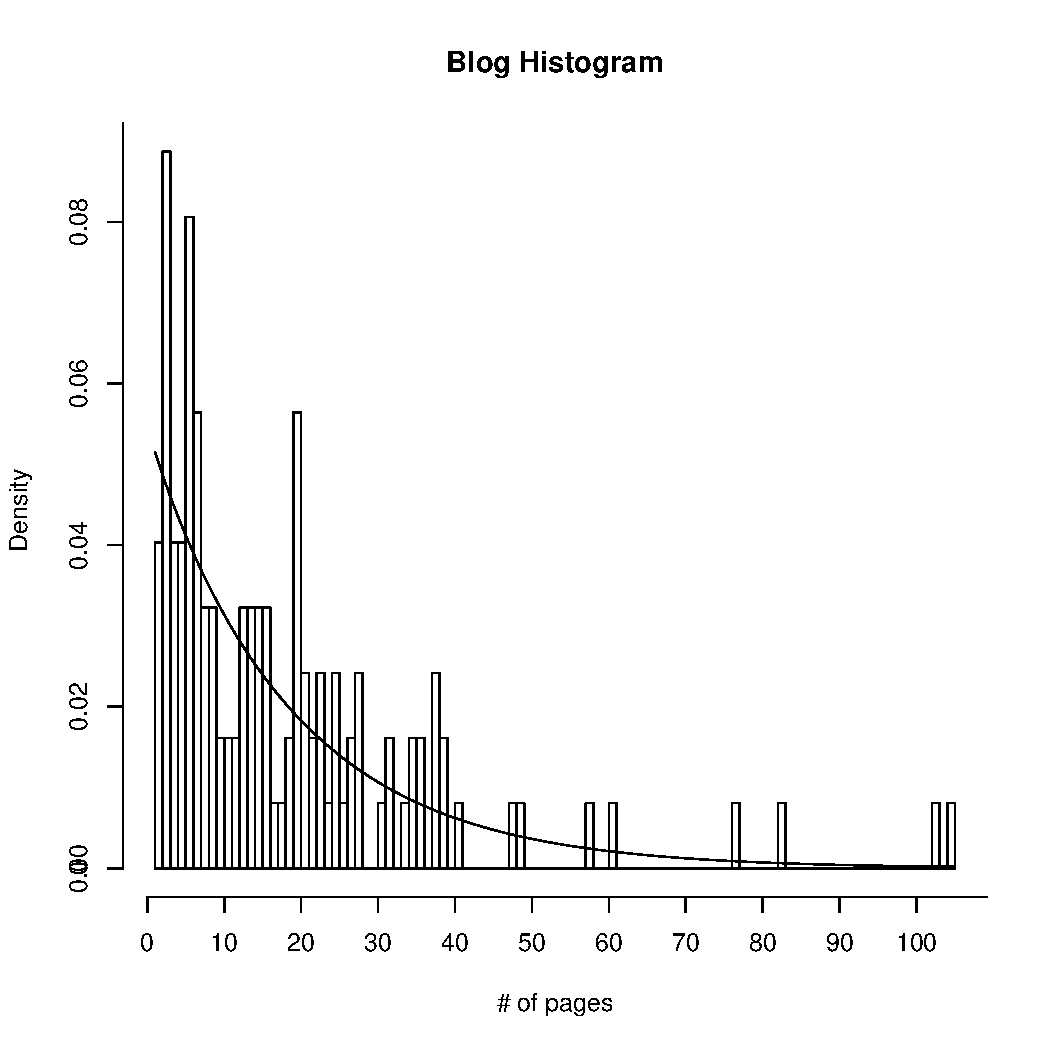
\includegraphics[width=.7\linewidth]{../q1/densHist.pdf}
  \caption{Probability Density Histogram (bins = no. blogs) with fitted Gamma distribution}
\end{figure}%



\begin{figure}
  \centering
  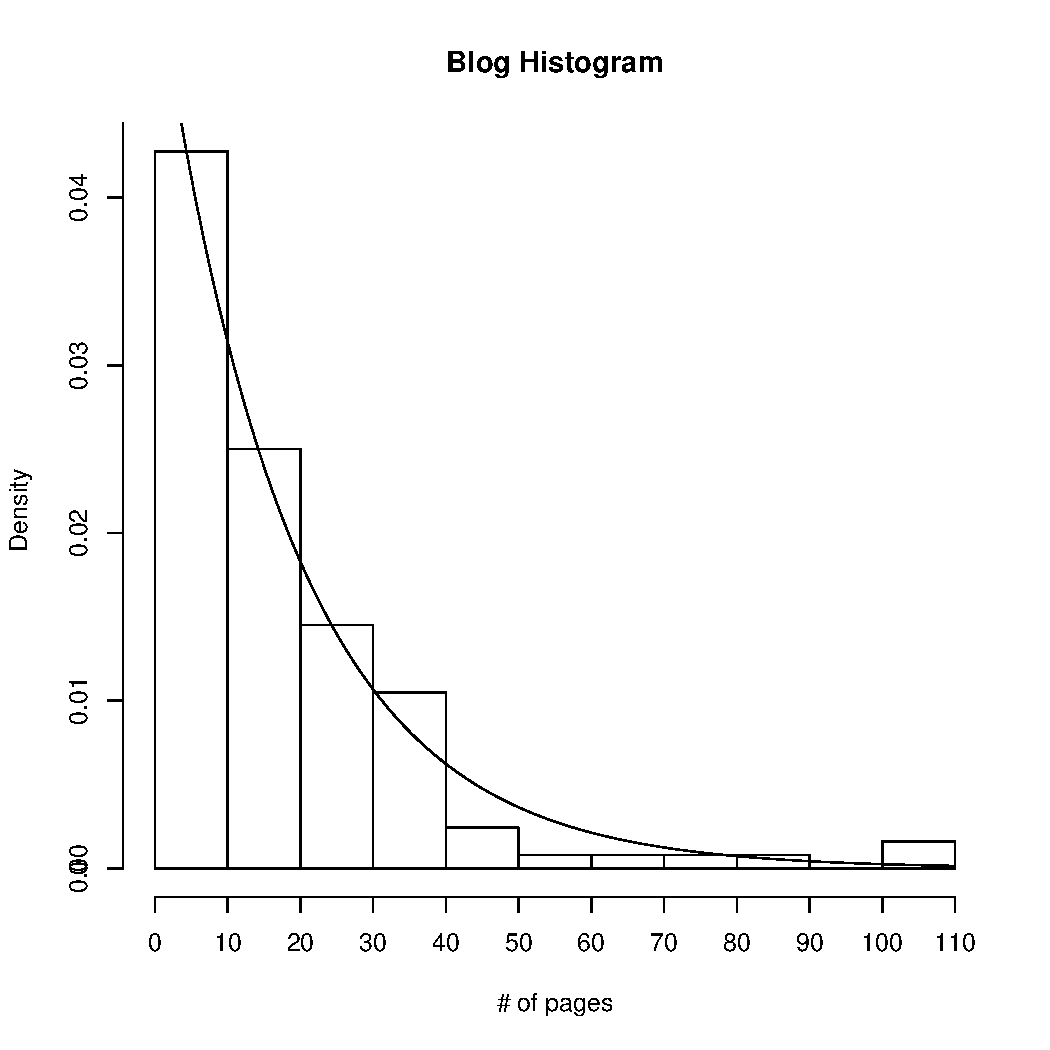
\includegraphics[width=.7\linewidth]{../q1/densHist1.pdf}
  \caption{Probability Density Histogram (bins = 10) with fitted Gamma distribution}
\end{figure}


